%===============================================================
\chapter{Game Development at FIT CTU}
%===============================================================

\begin{chapterabstract}	
    FIT CTU offers a robust Informatics programme with a specialisation in computer graphics, combining theoretical foundations with hands-on coursework in areas such as programming, visualization, and user interface design. The faculty regularly organises events like GameJams and supports a range of student-driven game projects, resulting in a diverse portfolio of innovative games. This chapter details the game development education, showcases notable student projects, and outlines the ecosystem of events that nurture game development at FIT CTU.
\end{chapterabstract}

The Faculty of Information Technology at the Czech Technical University (FIT~CTU) offers a range of courses and events dedicated to game development. Currently, only a single study programme is available---\textit{Informatics}---which includes several specialisations. Of particular relevance is the computer graphics specialisation, which combines theoretical foundations with practical experience. Core theoretical courses include \textit{Computer Graphics Programming}, \textit{Modern Visualisation Technologies}, \textit{Machine Vision}, and \textit{Image Processing}, while more hands-on experience is provided through courses such as \textit{Multimedia and Graphics Applications}, \textit{Programming of Graphic Applications}, and \textit{User Interface Design}.
\cite{fit_graphics}

Game development is also integrated into other CTU courses, such as Team Software Project, where students have the option to work on game-rated projects as part of their coursework.
\cite{FIT_courses}

In addition, FIT CTU is preparing a new study programme---\textit{Applied Informatics}---which will introduce three new specialisations: \textit{Game Development}, \textit{Graphics}, and \textit{Computer Vision}. This programme is expected to offer a stronger emphasis on practical experience and expand the number of study places available in game-related fields. As a result, a broader range of student-developed games is anticipated---many of which could benefit from structured entrepreneurial support.\footnote{Interview with Ing. Radek Richtr, Ph.D., guarantor of the computer graphics specialisation, conducted on 15 April 2025.}

The FIT GameJam—organised by Grafit—is another key event fostering game development. Held over an extended weekend, this 48-hour challenge tasks students with creating a computer game from scratch. Participants work either individually or in teams, and receive guidance from experienced industry professionals. The event cultivates teamwork, creativity, and showcases students’ technical and artistic talents.
\cite{grafit_itch}

Overall, multiple study paths at FIT CTU support the creation of original games---whether through specialised coursework, faculty-led research, extracurricular events, or student-driven initiatives. The faculty provides an environment in which aspiring developers can hone their skills and bring their ideas to life.

%===============================================================
\section{Example Games from FIT CTU}\label{sec:example-games}
Over the years, students at the FIT CTU have created a wide range of original, comical and technically impressive games. These projects often combine creative storytelling and original game mechanics and are developed as part of coursework, bachelor’s or master’s theses, GameJams or independent student initiatives.

\begin{figure}[H]
    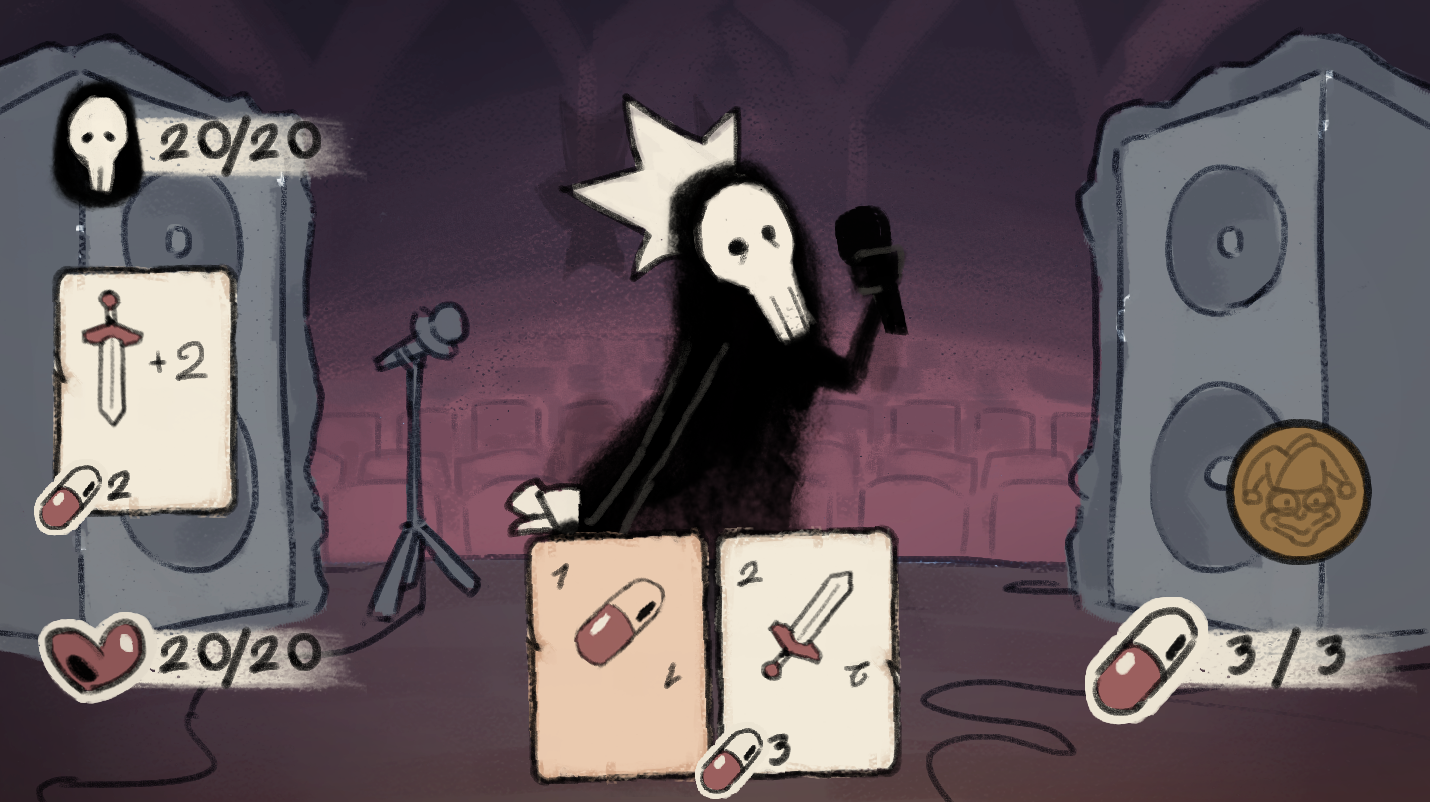
\includegraphics[width=0.9\textwidth]{encore.png}
    \caption{Image of Encore! from the GameJam's Itch.io~\cite{itch_encore}}
    \label{fig:encore-picture}
    Encore! developed during the 2024 GameJam by Belonzik and TheMultiplexx is a dueling  card game with an outstanding attention to detail exploring the theme of death. It stands out for its excellent graphics, well-crafted audio, immersive story and even professional-grade narration. \cite{itch_encore}
\end{figure}

\begin{figure}[H]
    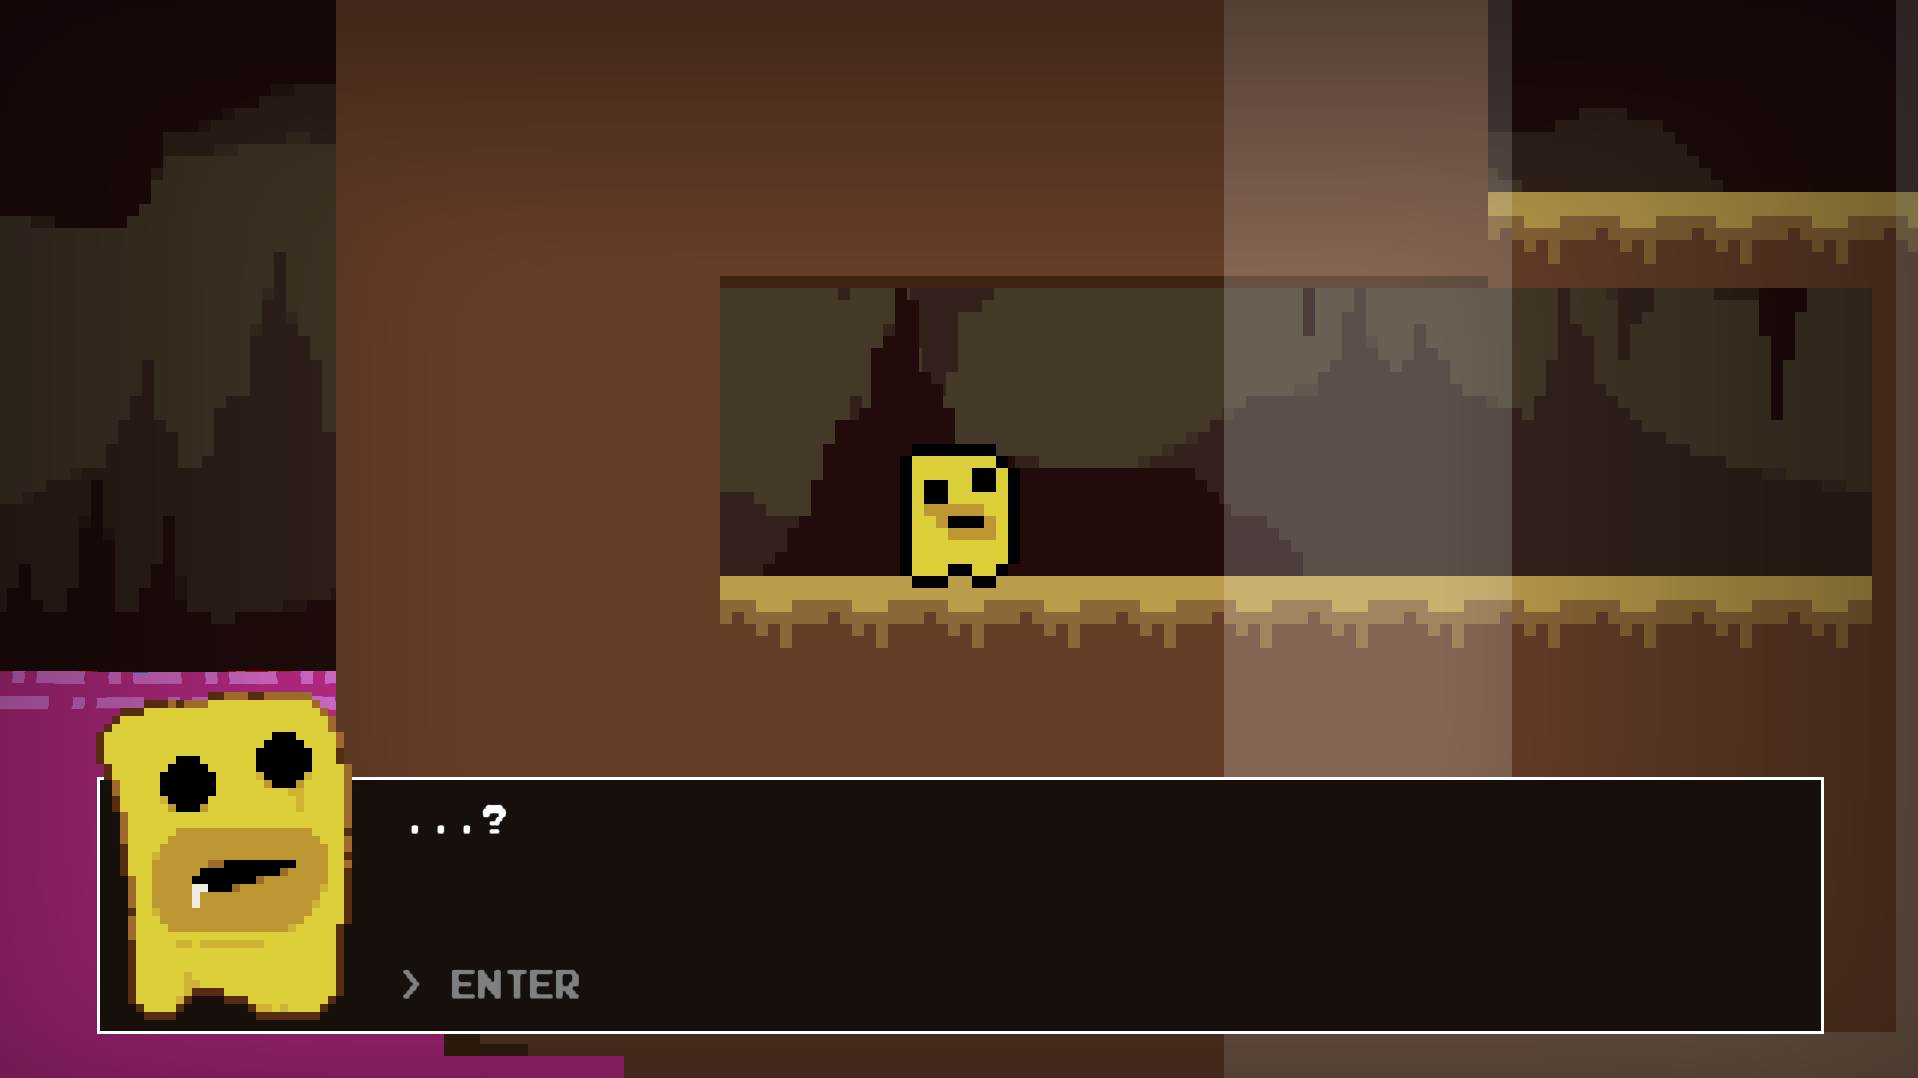
\includegraphics[width=0.9\textwidth]{liminal.png}
    \caption{Image of Liminal! from the GameJam's Itch.io~\cite{itch_liminal}}
    \label{fig:liminal-picture}
    Liminal! by HyperCubic Studio was developed during the 2024 GameJam too. This short platform puzzle game traps the player in a twisted TV show. The game’s colourful visuals are beautiful, cohesive and extensively polished. It boasts original mechanics and is full of details in the sounds, menu items and dialogue. \cite{itch_liminal}
\end{figure}

\begin{figure}[H]
    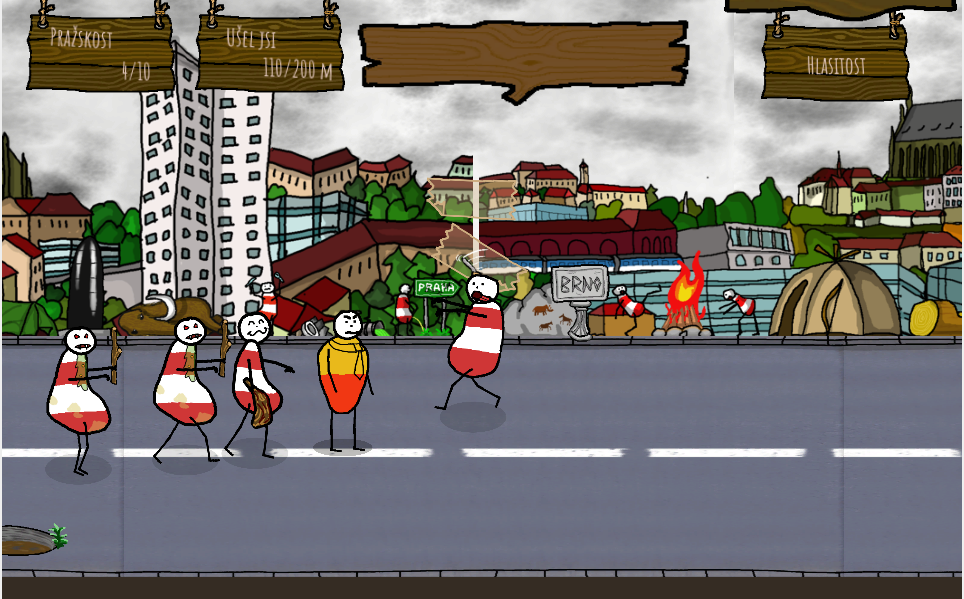
\includegraphics[width=0.9\textwidth]{brno.png}
    \caption{Image of Escape from Brno from the GameJam's Itch.io~\cite{itch_brno}}
    \label{fig:brno-picture}
    Escape from Brno was created during the 2022 GameJam by Trampod, SharpFoxDev, benjaminhejl, leia12321 and VAHAnima. This side-scrolling dodger won the popular vote. Its humorous sound design, cohesive graphics, and intuitive gameplay make it feel natural and engaging. \cite{itch_brno}
\end{figure}

\begin{figure}[H]
    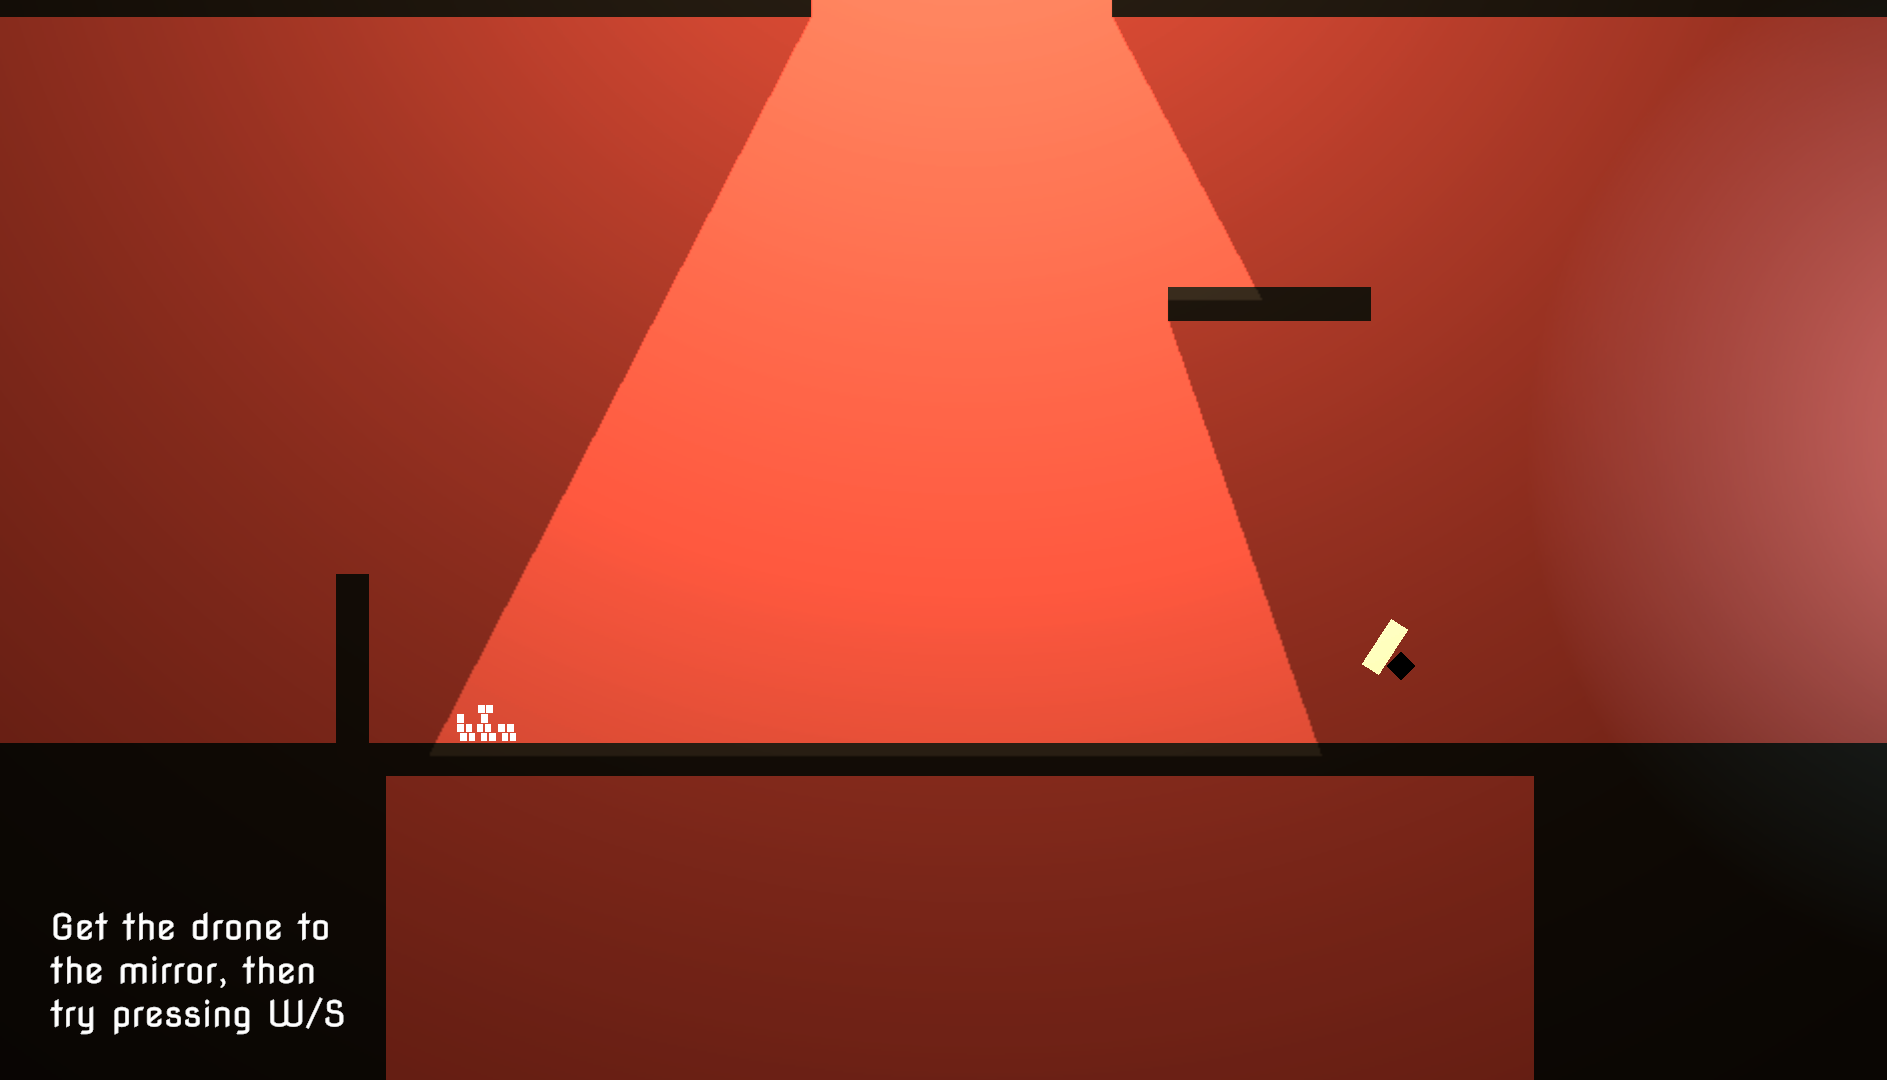
\includegraphics[width=0.9\textwidth]{subject.png}
    \caption{Image Subject 42 from the GameJam's Itch.io~\cite{itch_subject}}
    \label{fig:subject-picture}
    Subject 42 was created by LukyDrum during the 2023 GameHack. This game puts the player in control of a robot’s AI as they solve puzzles and navigate three intriguing levels. A fitting sound-track and a voice sarcastically commenting on the player’s performance contribute to its unique style and storytelling. \cite{itch_subject}
\end{figure}
